% !TEX root = main.tex

\section{优化算法}
\subsection{简介}
\begin{mini*}
    {}{f_0(x)}{}{}
    \addConstraint{A\vx}{=\vb}
\end{mini*}
罚函数法
\[\min f_0(x)+\frac{\lambda}{2}\norm{A\vx-\vb}_2^2\]
\[\tilde{x}=\arg\min_x F\]
\[\nabla f_0(\tilde{\lambda})+\lambda A^\T(A\tilde{\vx}-\vb)=0\]
\[\begin{aligned}
    L(x,v)&=f_0(x)+v^\T(A\vx-\vb)\\
    \implies g(v)&=\inf_x f_0(x)+v^\T(A\vx-\vb)\\
    v&=\lambda(A\tilde{\vx}-\vb)\\
    \implies & g(\lambda(A\tilde{x}-\vb)=\inf_x f_0(x)+\lambda(A\tilde{x}-b)^\T(A\vx-\vb)
\end{aligned}\]
\[\nabla f_0(x)+\lambda A^\T(A\tilde{x}-\vb)=0\]

\begin{mini*}
    {}{f_0(x)}{}{}
    \addConstraint{A\vx}{\geq\vb}
\end{mini*}
log-barrier
\[\min f_0(x)+\sum_{i=1}^m u_i\log(a_i^\T \vx-b_i)\]


$\min f_0(x)$可微,凸,无约束
\begin{enumerate}
    \item 所有算法都是迭代的
    \[\iter{x}{k+1}=\iter{x}{k}+\iter{\alpha}{k}\iter{d}{k}\]
    $\alpha\geq 0$为步长,$d$为方向,所有算法本质上都是选择方向与步长的问题
    \item 如何选择步长$\iter{\alpha}{k}$
    \[\begin{cases}
    \text{确定步长} & \begin{cases}\text{固定步长}\\\text{变化步长(递减步长)}\end{cases}\\
    \text{搜索步长}
    \end{cases}\]
    最优步长:线搜索问题
    \[\iter{\alpha}{k}=\arg\min_{\alpha\geq 0} f_0(\iter{x}{k}+\alpha\iter{d}{k})\]
    \item 关键问题是选方向
\end{enumerate}
黄金分割法(0.618法)/优选法求解线搜索问题:这样做的采样复杂度很低,之前算过的点很容易被再用!

不精确线搜索(Armijo Rule):一阶泰勒展开
% \begin{algorithm}[H]
%     \begin{algorithmic}[1]
%         \State{$\iter{\alpha}{k}=\alpha_\max$}
%         \If{$f_0(\iter{x}{k}+\iter{\alpha}{k}\iter{d}{k})>f_0(\iter{x}{k}+\mu\iter{\alpha}{k}\lrang{\nabla f_0(\iter{x}{k},\iter{d}{k})})$}
%         \State $\iter{\alpha}{k}\gets\iter{\alpha}{k}\beta,\beta\in(0,1)$
%         \Else
%         \State Stop
%         \EndIf
%     \end{algorithmic}
% \end{algorithm}

实际上没有必要求最优步长,在该方向上的差异并没有太大

\subsection{梯度下降法}
$\iter{d}{k}=-\nabla f_0(\iter{x}{k})$
\begin{itemize}
    \item 能否收敛
    \item 收敛到哪里
    \item 收敛速度
\end{itemize}

假设
\begin{itemize}
    \item[0.] 基本假设:$f$为可微的凸函数,
    \[x^\star=\arg\min_x f_0(x)\]
    存在且有限,$f_0(x^\star)$有限
    \item[1.] Lipschitz连续梯度
    \[\exists L\geq 0,\norm{\nabla f_0(x)-\nabla f_0(y)}\leq L\norm{x-y},\forall x,y\]
    等价定义:
    \begin{itemize}
        \item[a.]若$f_0(x)$二阶可微
    \[\nabla^2f_0(x)\preceq LI,\forall x\]
        \item[b.] 下界
    \[\lrang{\nabla f_0(x)-\nabla f_0(y),x-y}\geq\frac{1}{L}\norm{\nabla f_0(x)-\nabla f_0(y)}^2\]
        \item[c.] 上界
    \[\lrang{\nabla f_0(x)-\nabla f_0(y),x-y}\leq L\norm{x-y}\]
        \item[d.] 当函数为凸时
    \[0\leq f_0(y)-f_0(x)-\lrang{\nabla,y-x}\leq\frac{L}{2}\norm{x-y}_2^2\]
    \end{itemize}
    \item[2.] 强凸性(strong convexity)
    \[\exists\mu>0:\;f_0(y)\geq f_0(x)+\lrang{\nabla f_0(x),y-x}+\frac{\mu}{2}\norm{x-y}_2^2,\forall x,y\]
    二阶可微情况下的等价定义
    \[\nabla^2 f(x)\succeq \mu I\]
\end{itemize}
\begin{example}
    \[\begin{aligned}
        f_0(x) &= \vone^\T x\qquad & L &= 0 & \text{\xmark}\\
        f_0(x) &= \frac{1}{2}\norm{x}_2^2 & L &=1 & \mu=1\\
        f_0(x) &= \frac{1}{4}\norm{x}_2^4 & \text{\xmark} & &\text{\xmark}
    \end{aligned}\]
\end{example}

区别于严格凸(strictly convex),强凸一定是严格凸
\begin{theorem}
    严格凸函数只有一个最小值点
\end{theorem}
\begin{analysis}
    反证法,假设$x,y$均为最小值点,且$x\ne y$
    \[f_0(y)>f_0(x)+\lrang{\nabla f_0(x),x-y}=f_0(x)\]
\end{analysis}

\begin{theorem}
    若$f_0(x)$有Lipschitz连续梯度,常数$L$,若$\alpha\in(0,\frac{2}{L})$,则有
    \[\begin{aligned}
        f_0(\iter{x}{k})-f_0(x^\star)&\leq \frac{2(f_0(x^0)-f_0(x^\star))\norm{x^0-x^\star}^2}
        {2\norm{x^0-x^\star}^2+k\alpha(2-L\alpha)(f_0(x^0)-f_0(x^\star))},\forall x^\star
    \end{aligned}\]
    即以$O(\frac{1}{k})$速度收敛
\end{theorem}
\begin{analysis}
    $1\degree$ 点的单调性:与任意$x^\star$的距离在缩小
    \[\norm{\iter{x}{k+1}-x^\star}^2\leq\norm{\iter{x}{k}-x^\star}^2,\forall x^\star\]
    \[\begin{aligned}
        LHS &= \norm{\iter{x}{k}-x^\star-\alpha\nabla f_0(x^k)}^2\\
        &=\norm{\iter{x}{k}-x^\star}^2-2\alpha\lrang{x^k-x^\star,\nabla f_0(x^k)}+\alpha^2\norm{\nabla f_0(x^k)}\\
        &\leq \norm{\iter{x}{k}-x^\star}^2+\alpha(\alpha-\frac{2}{L})\norm{\nabla f_0(\iter{x}{k})}^2\qquad\text{注意到$\nabla f_0(x^\star)=0$,利用Lipschitz连续梯度}\\
        &\leq \norm{\iter{x}{k}-x^\star}^2
    \end{aligned}\]
    $2\degree$ 函数值的单调性:$f_0(\iter{x}{k+1})\leq f_0(\iter{x}{k})$(注意下降可能非常缓慢,并不一定收敛)
    \[\begin{aligned}
        f_0(\iter{x}{k+1})&\leq f_0(\iter{x}{k})+\lrang{\nabla f_0(\iter{x}{k}),\iter{x}{k+1}-\iter{x}{k}}+\frac{L}{2}\norm{\iter{x}{k+1}-\iter{x}{k}}^2\\
        &= f_0(\iter{x}{k})-\alpha(1-\frac{L\alpha}{2})\norm{\nabla f_0(\iter{x}{k})}^2\\
        &\leq f_0(\iter{x}{k})
    \end{aligned}\]
    $3\degree$ 函数值的充分下降(即证明收敛性)
    \[f_0(\iter{x}{k+1})-f_0(x^\star)\leq f_0(\iter{x}{k})-f_0(x^\star)-\omega\norm{\nabla f_0(\iter{x}{k})}^2\]
    \[\begin{aligned}
        f_0(\iter{x}{k})-f_0(x^\star)&\leq \lrang{f_0(\iter{x}{k},\iter{x}{k}-x^\star)}\\
        &=\lrang{\nabla f_0(\iter{x}{k})-\nabla f_0(x^\star),\iter{x}{k}-x^\star}\\
        &\leq\norm{\nabla f_0(\iter{x}{k})-\nabla f_0(x^\star)}\norm{\iter{x}{k}-x^\star}\\
        &\leq \norm{\nabla f_0(\iter{x}{k})}\norm{\iter{x}{k}-x^\star}
    \end{aligned}\]
    \[\iter{\Delta}{k+1}\leq \iter{\Delta}{k}-\frac{\omega}{\norm{x^0-x^\star}^2}(\iter{\Delta}{k})^2\]
    \[\frac{1}{\iter{\Delta}{k+1}}\leq\frac{1}{\iter{\Delta}{k+1}}-\frac{\omega}{\norm{x^0-x^\star}^2}\frac{\iter{\Delta}{k}}{\iter{\Delta}{k+1}}\]
    错位相消可得结论$O(\frac{1}{k})$收敛速度
\end{analysis}

\begin{theorem}
    若$f_0$有Lipschitz连续梯度,常数$L$,强凸函数$n$,步长$\alpha\in(0,\frac{2}{\mu+L}]$,则
    \[\norm{\iter{x}{k}-x^\star}^2\leq\lrp{1-\frac{2\alpha\mu L}{\mu+L}}^k\norm{\iter{x}{0}-x^\star}^2\]
\end{theorem}
\begin{analysis}
\[\begin{aligned}
    \norm{\iter{x}{k}-x^\star}^2 &= \norm{\iter{x}{k}-\alpha\nabla f_0(\iter{x}{k})-x^\star}^2\\
    &= \norm{\iter{x}{k}-x^\star}^2-2\alpha\lrang{\iter{x}{k}-x^\star,\nabla f_0(\iter{x}{k})}+\alpha^2\norm{\nabla f_0(\iter{x}{k})}^2\\
    &\leq \norm{\iter{x}{k}-x^\star}^2-\frac{2\alpha}{\mu+L}\norm{\nabla f_0(x)}^2+\alpha^2\norm{\nabla f_0(\iter{x}{k})}^2 \qquad\text{内积不等式}\\
    &\leq RHS
\end{aligned}\]
\[1-\frac{4\mu L}{(\mu+L)^2}=\frac{(L-\mu)^2}{(L+\mu)^2}=\frac{\lrp{\frac{L}{\mu}-1}^2}{\lrp{\frac{L}{\mu}+1}^2}\]
$L$为Hessian矩阵的最大特征值,$\mu$为Hessian矩阵的最小特征值,则$\frac{L}{\mu}$为该矩阵的条件数
\end{analysis}

不同收敛速度
\begin{itemize}
    \item 次线性收敛
    \item 线性收敛
    \item 超线性收敛
\end{itemize}
\begin{figure}[H]
    \centering
    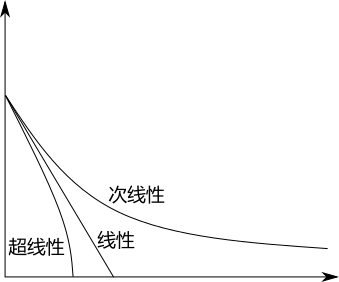
\includegraphics[width=0.3\linewidth]{fig/linear.png}
\end{figure}

\begin{example}
\[f_0(x)=\frac{1}{2}\norm{Ax-b}_2^2\]
\end{example}
\begin{analysis}
    \[\iter{x}{0}\to\iter{x}{1}\]
    \[\iter{x}{1}=\iter{x}{0}-\alpha(\iter{x}{0}-b)=b\]
\end{analysis}

条件数糟糕的病态矩阵收敛速度是非常糟糕的,会出现zig-zag的情况
\[A=\bmat{1 & 0\\ 0 & 10^{-4}}\]
可以通过预处理(precondition)来解决条件数糟糕的问题

$f_0$,Lipschitz连续梯度($L$),强凸($\mu$),函数值收敛性
\[\begin{aligned}
    \tilde{f}_0(\iter{\alpha}{k})&=f_0(\iter{x}{k+1})=f_0(\iter{x}{k}-\iter{\alpha}{k}\nabla f_0(\iter{x}{k}))\\
    &\leq f_0(\iter{x}{k})+\lrang{\nabla f_0(\iter{x}{k}),-\iter{\alpha}{k}\nabla f_0(\iter{x}{k})}+\frac{L}{2}\norm{-\iter{\alpha}{k}\nabla f_0(\iter{x}{k})}^2\\
    &=f_0(\iter{x}{k})+\frac{L(\iter{\alpha}{k})^2-2\iter{\alpha}{k}}{2}\norm{\nabla f_0(\iter{x}{k})}^2
\end{aligned}\]

$\iter{\alpha}{k}=\iter{\alpha}{k}_{exact}$精确线搜索
\[\begin{aligned}
    &\tilde{f}_0(\frac{1}{L})=f_0(\iter{x}{k})-\frac{1}{2L}\norm{\nabla f_0(\iter{x}{k})}^2\\
    &\tilde{f}_0(\iter{\alpha}{k}_{exact})\leq\tilde{f}_0(\frac{1}{L})\\
    \implies&\tilde{f}_0(\iter{\alpha}{k}_{exact})-f_0(\iter{x}{k})-f_0(x^\star)-\frac{1}{2L}\norm{\nabla f_0(\iter{x}{k})}^2\\
    &\leq (1-\frac{\mu}{L})(f_0(\iter{x}{k})+f_0(x^\star))
\end{aligned}\]
\[\begin{aligned}
    f_0(x^\star)&\geq f_0(\iter{x}{k})+\lrang{\nabla f_0(\iter{x}{k}),x^\star-\iter{x}{k}}+\frac{\mu}{2}\norm{\iter{x}{k}-x^\star}^2\\
    &\geq f_0(\iter{x}{k})-\frac{\mu}{2}\norm{\iter{x}{k}-x^\star}^2-\frac{1}{2\mu}\norm{\nabla f_0(\iter{x}{k})}^2+frac{\mu}{2}\norm{\iter{x}{k}-x^\star}^2\qquad ab\geq-\frac{\mu}{2}a^2-\frac{1}{2\mu}b^2\\
    &= f_0(\iter{x}{k})-\frac{1}{2\mu}\norm{\nabla f_0(\iter{x}{k})}^2
\end{aligned}\]
\[f_0(\iter{x}{k}-f_0(x^\star)\leq\frac{1}{2\mu}\norm{\nabla f_0(\iter{x}{k})}^2\]

Armijo Rule
\[\tilde{f}_0(\iter{\alpha}{k})=f_0(\iter{x}{k+1})\leq f_0(\iter{x}{k})+\frac{L(\iter{\alpha}{k})^2-2\iter{\alpha}{k}}{2}\norm{\nabla f_0(\iter{x}{k})}^2\]
\[\tilde{f}_0(\iter{\alpha}{k})=f_0(\iter{x}{k+1})\leq f_0(\iter{x}{k})-\nabla\iter{\alpha}{k}\norm{\nabla f_0(\iter{x}{k})}^2\]
首先说明,若$0\leq\iter{\alpha}{k}\leq\frac{1}{L}$时,则
\[\tilde{f}_0(\iter{\alpha}{k})\leq f_0(\iter{x}{k})-\gamma\iter{\alpha}{k}\norm{\nabla f_0(\iter{x}{k})}^2\]
当$\iter{\alpha}{k}\in[0,\frac{1}{2}]$时,
\[-\iter{\alpha}{k}+\frac{L}{2}(\iter{\alpha}{k})^2\leq -\frac{\iter{\alpha}{k}}{2}\iff \frac{L}{2}(\iter{\alpha}{k})^2\leq\frac{\iter{\alpha}{k}}{2}\iff L\cdot\iter{\alpha}{k}\leq 1\]
\[\begin{aligned}
    f_0(\iter{x}{k+1})&\leq f_0(\iter{x}{k})+\frac{L(\iter{\alpha}{k})^2-2\iter{\alpha}{k}}{2}\norm{\nabla f_0(\iter{x}{k})}^2\\
    &\leq f_0(\iter{x}{k})-\frac{\iter{\alpha}{k}}{2}\norm{\nabla f_0(\iter{x}{k})}^2\\
    &\leq f_0(\iter{x}{k})-\gamma\iter{\alpha}{k}\norm{\nabla f_0(\iter{x}{k})}^2
\end{aligned}\]
\[\begin{aligned}
    &f_0(\iter{x}{k+1})\leq f_0(\iter{x}{k})-\min\{\gamma\alpha_{\max},\frac{\gamma\beta}{L}\}\norm{\nabla f_0(\iter{x}{k})}^2\\
    &\implies f_0(\iter{x}{k+1})-f_0(x^\star)\leq\lrp{1-\min\{2\mu\gamma\alpha_{\max},\frac{2\mu\gamma\beta}{L}\}}(f_0(\iter{x}{k}-f_0(x^\star)))
\end{aligned}\]

梯度下降法的解释1
\[\iter{x}{k+1}=\iter{x}{k}-\iter{\alpha}{k}\nabla f_0(\iter{x}{k})\]
将$f_0$在$\iter{x}{k}$处进行一阶Taylor展开
\[f_0(x)\approx f_0(\iter{x}{k})+\lrang{\nabla f_0(\iter{x}{k}),x-\iter{x}{k}}+\frac{1}{2\iter{\alpha}{k}}\norm{x-\iter{x}{k}}^2\]
求梯度
\[\begin{aligned}
    \nabla f_0(\iter{x}{k})+\frac{1}{\iter{\alpha}{k}}(x-\iter{x}{k})&=0\\
    \iter{\alpha}{k}\nabla f_0(\iter{x}{k})+x-\iter{x}{k}&=0\\
    x=\iter{x}{k}&-\iter{\alpha}{k}\nabla f_0(\iter{x}{k})
\end{aligned}\]

解释2
\[f_0(\iter{x}{k}+v)\approx f_0(\iter{x}{k})+\lrang{\nabla f_0(\iter{x}{k}),v}\]
\[\iter{d}{k}=\arg\min_v\{\lrang{\nabla f_0(\iter{x}{k}),v}\mid \norm{v}=1\}\]
若采用2-范数,可得标准化的负梯度方向(normalized negative gradient)
\[\iter{d}{k}=\frac{-\nabla f_0(\iter{x}{k})}{\norm{\nabla f_0(\iter{x}{k}}_2}\]
通过改变不同的范数,有不同的特性

坐标下降法(coordinate descent/alternating direction)交替极小化
\[\iter{d}{k}=\ve_{\mod{}{}}(k,n)\]
注意,这里$x\in\rn$,$n \mod n = n$
\[\iter{\alpha}{k}=\arg\min f_0(\iter{x}{k}+\alpha\iter{d}{k}),\alpha_{\max}\geq \alpha\geq \alpha_{\min}\]

\subsection{非光滑优化问题}
\subsubsection{次梯度法}
\[\min f_0(x),\qquad f_0\text{连续,凸,不可微}\]
梯度\textbf{下降}法$\to$次梯度(subgradient)法\\
$g_0(x)\in\partial f_0(x)$(注意凹函数则对应的是supgradient)
\[f_0(y)\geq f_0(x)+\lrang{g_0(x),y-x},\forall y\]
$f(x)=|x|$在零点处次梯度为$[-1,1]$
\[\iter{x}{k+1}=\iter{x}{k}-\iter{\alpha}{k}g_0(\iter{x}{k})\]
只要有$0\in\partial f_0(x_0)$就有最优解$x=x_0$

如果激活函数为非光滑的(如ReLU),那么出来的函数也是非光滑的,就要用次梯度

关键在于选择步长
\begin{itemize}
    \item 固定步长$\iter{\alpha}{k}=\alpha$
    \item 不可加但平方可加,如$\frac{1}{k}$
    \[\sum_{k=0}^\infty \iter{\alpha}{k}=\infty\qquad\sum_{k=0}^\infty(\iter{\alpha}{k})^2<\infty\]
    \item 不可加递减,如$\frac{1}{\sqrt{k}}$
    \[\sum_{k=0}^\infty\iter{\alpha}{k}=0\qquad\lim_{k\to\infty}\iter{\alpha}{k}\to 0\]
\end{itemize}

\[\inf_{i=0,\ldots,k}(f_0(\iter{x}{i})-f_0(x^\star))\]
\[\iter{\bar{x}}{k}:=\frac{\sum_{i=0}^k\iter{\alpha}{i}\iter{x}{i}}{\sum_{i=0}^k\iter{\alpha}{i}}\]
\[f_0(\iter{\bar{x}}{k})-f_0(x^\star)\]

假设函数Lipschitz连续
\[\exists G>0,\forall x,y:\;\norm{f_0(x)-f_0(y)}\leq G\norm{x-y}\]
$\forall x^\star$最优
\[\begin{aligned}
    &\qquad\norm{\iter{x}{k+1}-x^\star}^2=\norm{\iter{x}{k}-\iter{\alpha}{k}g_0(\iter{x}{k})-x^\star}^2\\
    &=\norm{\iter{x}{k}-x^\star}^2-2\lrang{\iter{\alpha}{k}g_0(\iter{x}{k}),\iter{x}{k}-x^\star}+(\iter{\alpha}{k})^2\norm{g_0(\iter{x}{k})}^2\\
    &\leq \norm{\iter{x}{k}-x^\star}^2-2(\iter{\alpha}{k})^2(f_0(\iter{x}{k})-f_0(x^\star))+(\iter{\alpha}{k})^2 G^2\\
    &\implies \norm{\iter{x}{k+1}-x^\star}^2\leq \norm{\iter{x}{0}-x^\star}^2-2\sum_{i=0}^k\iter{\alpha}{i}(f_0(\iter{x}{i})-f_0(x^\star))+\sum_{i=0}^k(\iter{\alpha}{i})^2 G^2\\
    &\implies 2\sum_{i=0}^k\iter{\alpha}{i}(f_0(\iter{x}{i})-f_0(x^\star))\leq \norm{\iter{x}{0}-x^\star}^2+\sum_{i=0}^k(\iter{\alpha}{i})^2G^2
\end{aligned}\]
\[\sum_{i=0}^k\iter{\alpha}{i}(f_0(\iter{x}{i})-f_0(x^\star))\geq\lrp{\sum_{i=0}^k\iter{\alpha}{i}}\inf_{i=0,\ldots,k}(f_0(\iter{x}{i})-f_0(x^\star))\]
\[\implies\inf_{i=0,\ldots,k}(f_0(\iter{x}{i})-f_0(x^\star))\leq\frac{\norm{\iter{x}{0}-x^\star}^2+G^2\sum_{i=0}^k(\iter{\alpha}{i})^2}{2\sum_{i=0}^k\iter{\alpha}{i}}\]
这是一个紧的界
\begin{itemize}
    \item 固定步长得到上界$\frac{G^2\alpha}{2}$,以$f(x)=|x|$为例
    \item 不可加平方可加一定收敛,若步长为$\frac{1}{k}$,收敛速度为$\frac{1}{\log k}$(幂级数积分取上下界$\sum_{i=0}^k\frac{1}{i}=O(\log k)$)
    \item 不可加平方不可加同样收敛,若步长为$\frac{1}{\sqrt{k}}$,收敛速度为$O(\frac{\log k}{\sqrt{k}})$,可以证明在该假设下该收敛速度最优
\end{itemize}

\[\lim_{k\to\infty}\inf_{i=0,\ldots,k}\lrp{f_0(\iter{x}{i})-f_0(x^\star)}=0\]
\[\forall \eps>0,\exists N_1\in\zz, \iter{\alpha}{i}\leq\frac{\eps}{G^2},\forall i>N_1\]
\[\exists N_2\in\zz:\sum_{i=0}^k\iter{\alpha}{i}\geq\frac{1}{\eps}\lrp{\norm{\iter{x}{0}-x^\star}^2+G^2\sum_{i=0}^{N_1}(\iter{\alpha}{i})^2},\forall k>N_2\]
另$N=\max\{N_1,N_2\},\forall k>N$
\[\frac{\norm{\iter{x}{0}-x^\star}^2+G^2\sum_{i=0}^{N_1}(\iter{\alpha}{i})^2}{2\sum_{i=0}^k\iter{\alpha}{i}}+\frac{\norm{\iter{x}{0}-x^\star}^2+G^2\sum_{i=N_1+1}^{k}(\iter{\alpha}{i})^2}{2\sum_{i=0}^{N_1}\iter{\alpha}{i}+2\sum_{i=N_1+1}^{k}\iter{\alpha}{i}}\leq\frac{\eps}{2}+\frac{\eps}{2}=\eps\]
\[\text{第二项}\leq\frac{G^2\sum_{i=N_1+1}^k\iter{\alpha}{i}\frac{\eps}{G^2}}{2\sum_{i=0}^{N_1}\iter{\alpha}{i}+2\sum_{i=N_1+1}^{k}\iter{\alpha}{i}}\leq\frac{\eps}{2}\]
实际上这个假设一般情况下不成立,但是我们只需保证在优化路径上成立即可,也有设置$x$有界的

\subsubsection{邻近点梯度法(proximal gradient method)}
有\textbf{结构},不可微

\[\min f_0(x)=s(x)+r(x)\]
\begin{itemize}
    \item s: smooth,可微,易求导
    \item r: regularization,不可微,易求邻近点投影
\end{itemize}

\[r(x),\hat{x}\cdot\alpha>0\]
邻近点投影(proximal mapping)
\[\min_x r(x)+\frac{1}{2\alpha}\norm{x-\hat{x}}^2\]
\begin{example}[LASSO]
    \[f_0(x)=\frac{1}{2}\norm{y-Ax}^2+\lambda\norm{x}_1\]
\end{example}
\begin{analysis}
    本来想优化0-范数,但因为不好做,故变为优化1-范数
    \[\arg\min\lambda\norm{x}_1+\frac{1}{2\alpha}\norm{x-\hat{x}}^2\]
    Hessian矩阵是单位阵,好解得多
    \[\lambda\sum_{i=1}^n\norm{x_i}+\frac{1}{2\alpha}\sum_{i=1}^n(x_i-\hat{x}_i)^2\]
    由于每一维并没有耦合在一起,因此相当于每一个维度都最优化
    \[\arg\min\lambda |x_i|+\frac{1}{2\alpha}(x_i-\hat{x}_i)^2\] % 考试!
    \[0\in\lambda\partial|x_i|+\frac{1}{\alpha}(x_i-\hat{x}_i)\]
    \begin{enumerate}
        \item 若$x_i>0$,则
        \[0=\lambda+\frac{1}{\alpha}(x_i-\hat{x}_i)\]
        \[\implies x_i=\hat{x}_i-\alpha\lambda,\hat{x}_i>\alpha\lambda\]
        \item 若$x_i<0$,则
        \[0=-\lambda+\frac{1}{\alpha}(x_i-\hat{x}_i)\]
        \[\implies x_i=\hat{x}_i+\alpha\lambda,\hat{x}_i<\alpha\lambda\]
        \item 若$x_i=0$,则
        \[0\in[-\lambda,\lambda]-\frac{1}{\alpha}\hat{x}_i\implies 0\in[-\lambda-\frac{1}{\alpha}\hat{x}_i,\lambda-\frac{1}{\alpha}\hat{x}_i]\]
        \[0\geq -\lambda-\frac{1}{\alpha}\hat{x}_i\implies \hat{x}_i\geq -\lambda\alpha,\hat{x}_i\leq\lambda\alpha\]
    \end{enumerate}
    画软门限(soft thresholding)图,横轴$\hat{x}_i$,纵轴$x_i$
    \begin{itemize}
        \item $\iter{x}{k+\frac{1}{2}}=\iter{x}{k}-\alpha A^\T (A\iter{x}{k}-y)$
        \item $\iter{x}{k}=\arg\min_x\lambda\norm{x}_1+\frac{1}{2\alpha}\norm{x-\iter{x}{\frac{1}{2}}}^2$
    \end{itemize}
    即ISTA算法
\end{analysis}

\begin{example}[盒限制(box constrained)优化问题]
\[f_0(x)=s(x)+\sum_{i=1}^nI(x_i\in[l_i,u_i])\]
\end{example}
\begin{analysis}
\[\begin{aligned}
    \qquad\arg\min r(x)+\frac{1}{2\alpha}\norm{x-\hat{x}}^2\\
    &=\arg\min\frac{1}{2\alpha}\norm{x-\hat{x}}^2\\
    &\text{s.t.}\forall i, x_i\in[l_i,u_i]
\end{aligned}\]
如果有约束$x\in\sC$
\begin{itemize}
    \item $\iter{x}{k+\frac{1}{2}}=\iter{x}{k}-\alpha\nabla S(\iter{x}{k})$
    \item $\iter{x}{k+1}=\arg\min_x I_\sC(\iter{x}{k+\frac{1}{2}})+\frac{1}{2\alpha}\norm{x-\iter{x}{k+\frac{1}{2}}}^2=\arg\min_x\frac{1}{2\alpha}\norm{x-\iter{x}{k+\frac{1}{2}}}^2,x\in\sC$
    \item 相当于做投影,故称投影梯度法
\end{itemize}
\end{analysis}

\[\iter{x}{k+\frac{1}{2}}=\iter{x}{k}-\alpha\nabla S(\iter{x}{k})\]
\[\iter{x}{k}=\arg\min_x r(x)+\frac{1}{2\alpha}\norm{x-\iter{x}{k+\frac{1}{2}}}^2\]
\[\begin{aligned}
    0&\in\partial r(\iter{x}{k+1})+\frac{1}{\alpha}(\iter{x}{k+1}-\iter{x}{k+\frac{1}{2}})\\
    0&=\partial r(\iter{x}{k+1})+\frac{1}{\alpha}(\iter{x}{k+1}-\iter{x}{k}+\alpha\nabla S(\iter{x}{k}))\\
    \iter{x}{k+1}&=\iter{x}{k}-\alpha\nabla S(\iter{x}{k})-\alpha\partial r(\iter{x}{k+1})
\end{aligned}\]
数值计算:显式方法(次梯度法)$\to$隐式方法(邻近点梯度法---需要先知道下一步信息,但是这是可以做的,因为有邻近点)

收敛性能与梯度下降法类似

\begin{example}[矩阵补全]
    $Y\in\rr^{m\times n},\{Y_{ij},(i,j)\in\Omega\}$
    \[\min_B\frac{1}{2}\sum_{(i,j)\in\Omega}(Y_{ij}-B_{ij})^2+\lambda\oprank(B)\]
\end{example}
\begin{analysis}
    同LASSO,由于矩阵的秩(奇异值向量0-范数)不好求,改为矩阵的和范数$\norm{\cdot}$(奇异值向量1-范数),即
    \[\min_B\frac{1}{2}\sum_{(i,j)\in\Omega}(Y_{ij}-B_{ij})^2+\lambda\norm{B}_\star\]
    \[\norm{B}_\star:=\sum_{i=1}^n\sigma_i(B)\]
    \[\min\frac{1}{2}\norm{P_\Omega(B-Y)}_F^2+\lambda\norm{B}_\star\]
    其中$P_\Omega$为$0$,若原矩阵中该项不存在;存在的话则保持不变
    \[\nabla B(\frac{1}{2}\norm{P_\Omega}(B-Y)_F^2)=P_\Omega(B-Y)\]
    对$B$做奇异值分解,$U$为酉矩阵
    \[\partial\norm{B}_\star=\{UDV^\T, B=U\Sigma V^\T, d=\partial\norm{\sigma}_1\}\]
    \begin{itemize}
        \item $\iter{B}{k+\frac{1}{2}}=B^k-\alpha P_\Omega(B^k-Y)$
        \item $\iter{B}{k+1}=\arg\min_B\lambda\norm{B}_\star+\frac{1}{2\alpha}\norm{B-\iter{B}{k+\frac{1}{2}}}_F^2$
    \end{itemize}
    \[0\in\lambda\partial\norm{B}_\star+\frac{1}{\alpha}(B-\iter{B}{k+\frac{1}{2}})\]
    \[0\in[\lambda UDV^\T+\frac{1}{\alpha}(B-\iter{B}{k+\frac{1}{2}})]\]
    \[B=U\Sigma V^\T,\;d=\partial\norm{\sigma}_1\]
    \[0\in\{\lambda UDV^\T +\frac{1}{\alpha}(V\Sigma V^\T-\iter{B}{k+\frac{1}{2}})\}\]
    \[\exists V,0=\alpha\lambda UDV^\T+V\Sigma V^\T-\iter{B}{k+\frac{1}{2}}\]
    \[\iter{B}{k+\frac{1}{2}}=U(\alpha\lambda D+\Sigma)V^\T\]
    对$\iter{B}{k+\frac{1}{2}}$进行奇异值分解
    \[\iter{B}{k+\frac{1}{2}}=U\iter{\Sigma}{k+\frac{1}{2}}V\]
    \[T_i=\alpha\lambda d_i+\sigma_i\]
    若$\sigma_i\ne 0\implies \tau_i=\alpha\lambda+\sigma_i$\\
    若$\sigma_i=0\implies \tau_i\in[-\alpha\lambda+\sigma_i,\alpha\lambda+\sigma_i]$\\
    \[\begin{cases}
        \sigma_i=\tau_i-\alpha\lambda & \tau_i>\alpha\lambda\\
        \sigma_i=0 & \tau_i\leq\alpha\lambda
    \end{cases}\]
    该算法称为矩阵软门限(soft thresholding)算法
\end{analysis}

一阶方法总结:
\begin{itemize}
    \item 梯度下降法
    \item 次梯度法:在随机/不确定性优化问题中很有效
    \item 邻近点梯度法
\end{itemize}